\documentclass[12pt,titlepage]{article}
\usepackage[margin=1.25in]{geometry}
\usepackage{graphicx,amsmath,blindtext,minted}

%% Variables definition
\newcommand{\vSubject}{Basic Programming Practicum}
\newcommand{\vSubtitle}{Jobsheet 5 Selection 2}
\newcommand{\vName}{Dicha Zelianivan Arkana}
\newcommand{\vNIM}{2241720002}
\newcommand{\vClass}{1i}
\newcommand{\vDepartment}{Information Technology}
\newcommand{\vStudyProgram}{D4 Informatics Engineering}

%% [START] Tikz related stuff
\usepackage{tikz}
\usetikzlibrary{svg.path,calc,shapes.geometric,shapes.misc}
\tikzstyle{terminator} = [rectangle, draw, text centered, rounded corners = 1em, minimum height=2em]
\tikzstyle{preparation} = [chamfered rectangle, chamfered rectangle sep=0.75em, draw, text centered, minimum height = 2em]
\tikzstyle{process} = [rectangle, draw, text centered, minimum height=2em]
\tikzstyle{decision} = [diamond, aspect=2, draw, text centered, minimum height=2em]
\tikzstyle{data}=[trapezium, draw, text centered, trapezium left angle=60, trapezium right angle=120, minimum height=2em]
\tikzstyle{connector} = [line width=0.25mm,->]
%% [END] Tikz related stuff

%% [START] Fancy header related stuff
\usepackage{fancyhdr}
\pagestyle{fancy}
\setlength{\headheight}{15pt} % compensate fancyhdr style
\fancyhead{}
\fancyfoot{}
\fancyfoot[L]{\thepage}
\fancyfoot[R]{\textit{\vSubject - \vSubtitle}}
\renewcommand{\footrulewidth}{0.4pt}% default is 0pt, overline for footer
%% [END] Fancy header related stuff

%% [START] Custom tabular command related stuff
\usepackage{tabularx}
\newcommand{\details}[2]{
    #1 & #2  \\
}
%% [END] Custom tabular command related stuff

%% [START] Figure related stuff
\newcommand{\image}[3][1]{
    \begin{figure}[h]
        \centering
        \includegraphics[#1]{#2}
        \caption{#3}
        \label{#3}
    \end{figure}
}
%% [END] Figure related stuff

\begin{document}
\begin{titlepage}
    \centering
    \vfill
    {\bfseries\LARGE
        \vSubject\\
        \vskip0.25cm
        \vSubtitle
    }
    \vfill
    
\includegraphics[width=6cm]{images/polinema-logo.png}
    \vfill
    {
        \textbf{Name}\\
        \vName\\
        \vskip0.5cm
        \textbf{NIM}\\
        \vNIM\\
        \vskip0.5cm
        \textbf{Class}\\
        \vClass\\
        \vskip0.5cm
        \textbf{Department}\\
        \vDepartment\\
        \vskip0.5cm
        \textbf{Study Program}\\
        \vStudyProgram
    }
\end{titlepage}

\tableofcontents

\pagebreak

\section{Laboratory}
\subsection{Experiment 1}

\begin{enumerate}
    \item Open a text editor. Create a new file, name it \textbf{Nested1.java}
    \item Write the basic structure of the Java programming language which contains the \texttt{main()} function
    \item Add the \texttt{Scanner} library.
    \item Make a \texttt{Scanner} declaration with the name sc
    \item Create an \texttt{int} variable with the name \texttt{value}
    \item {
        Write down the syntax for entering the value from keyboard

        \begin{minted}[autogobble,fontsize=\small]{java}
            System.out.print("Enter a value (0 - 100): ");
            value = sc.nextInt();
        \end{minted}
    }
    \item {
        Create a nested selection structure. The first check is used to ensure that the value
        entered is in the range 0 - 100. If the value is in the range 0 - 100, then a student
        graduation status will be checked, i.e. if the value is between 90 - 100 then the value is
        A, if the value is between 80 - 89 then the value is B, if the value is between 60 - 79 then
        the value is C, if the value is between 50 - 59 then the value is D, and if the value is
        between 0 - 49 then the value is E. Whereas if the value is outside the range 0 - 100 , then
        displayed information stating that the value entered is invalid.

        \begin{minted}[autogobble,fontsize=\small]{java}
            if (value >= 0 && value <= 100) {
                if (value >= 90 && value <= 100) {
                    System.out.println("Grade A, EXCELLENT!");
                } else if (value >= 80 && value <= 89) {
                    System.out.println("Grade B, keep up your achievements!");
                } else if (value >= 60 && value <= 79) {
                    System.out.println("Grade C, increase your achievements!");
                } else if (value >= 50 && value <= 59) {
                    System.out.println("Grade D, improve your study!");
                } else {
                    System.out.println("Grade E, you don't pass!");
                }
            } else {
                System.out.println("The value you entered is invalid");
            }
        \end{minted}
    }
    \pagebreak
    \item {
        Compile and run the program. Observe the results!

        \begin{figure}[h]
            \centering
            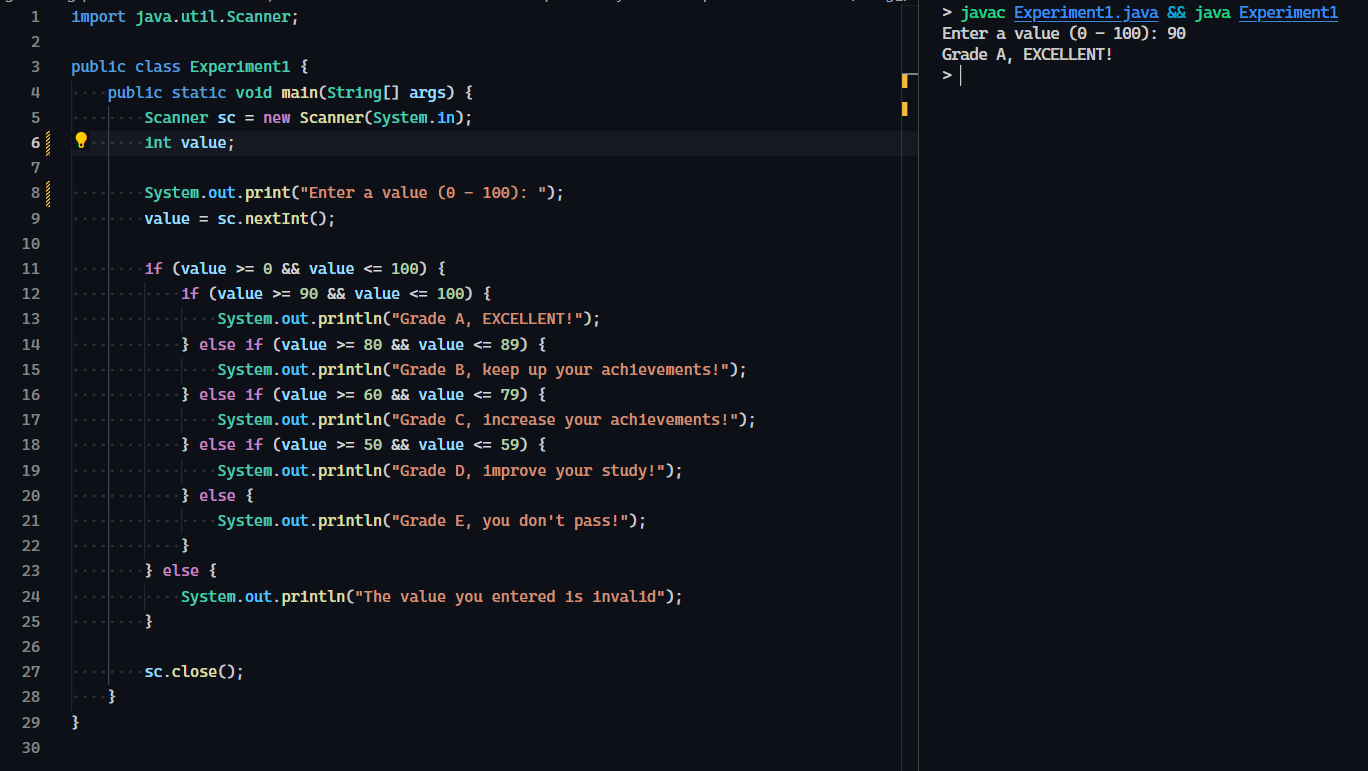
\includegraphics[width=\textwidth]{images/experiment1.png}
            \caption{Experiment 1 Code and Output}
        \end{figure}
    }
\end{enumerate}
\subsection*{Questions}
\begin{enumerate}
    \item {
        Describe the following syntax functions!
        \begin{minted}[autogobble,fontsize=\small]{java}
            if (value >= 0 && value <= 100)
        \end{minted}
        This syntax means that we're checking if \texttt{value} is greater than equal to 0 and it's less than equal to 100.
    }
    \pagebreak
    \item {
        Modify the program code in Experiment 1 so that if the entered value is less than 0 the
        output "Value you entered is less than 0" and if the entered value is more than 100 the
        output will display "The value you entered is more than 100"!

        \begin{figure}[h]
            \centering
            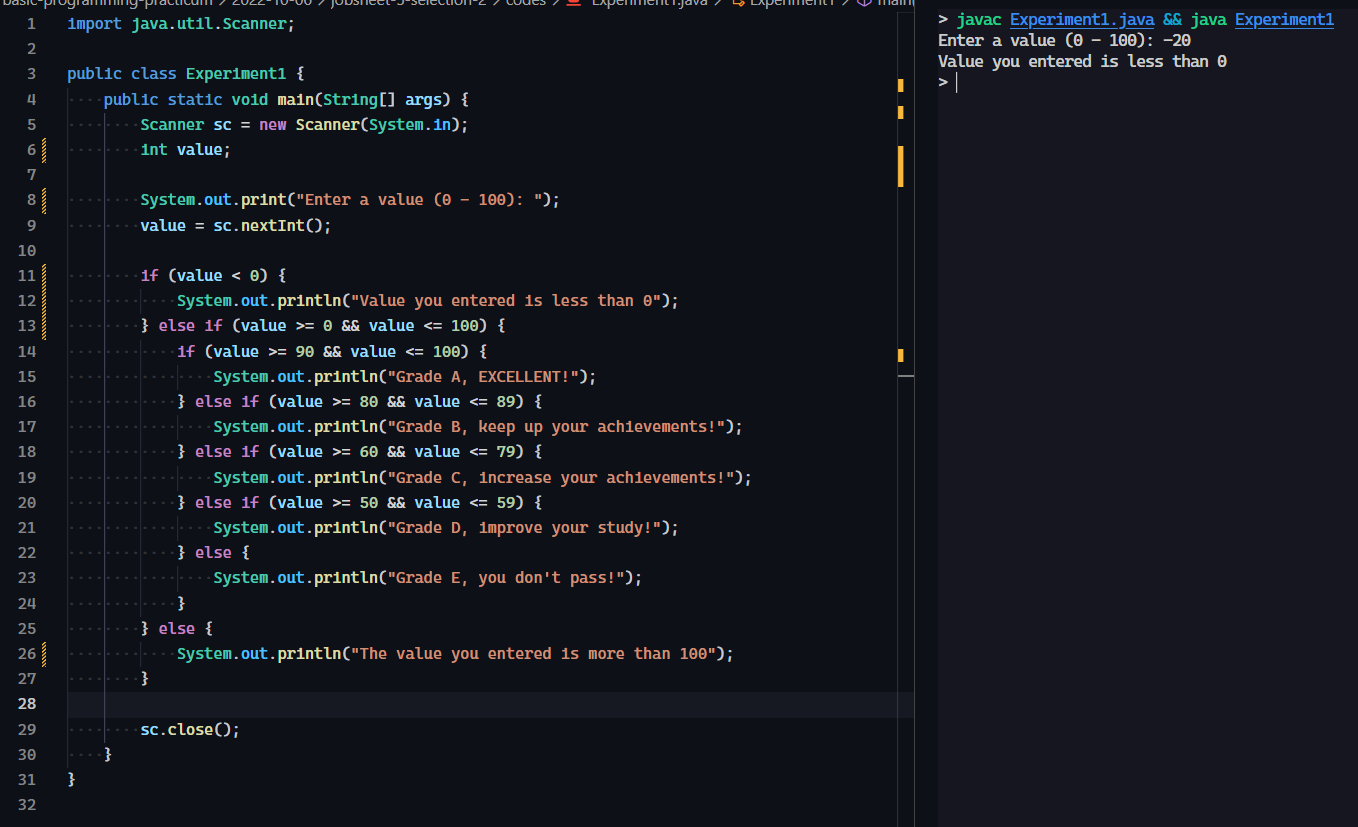
\includegraphics[width=\textwidth]{images/experiment1-modified.png}
            \caption{Experiment 1 Modified Code and Output}
        \end{figure}
    }
    \pagebreak
    \item {
        Change the \texttt{\&\&} operator to \texttt{||} on \texttt{if (value >= 0 \&\& value <= 100)}. Compile
        and run the program by entering the value = 105 using keyboard. Watch what happened!
        Why is the result like that?

        \begin{figure}[h]
            \centering
            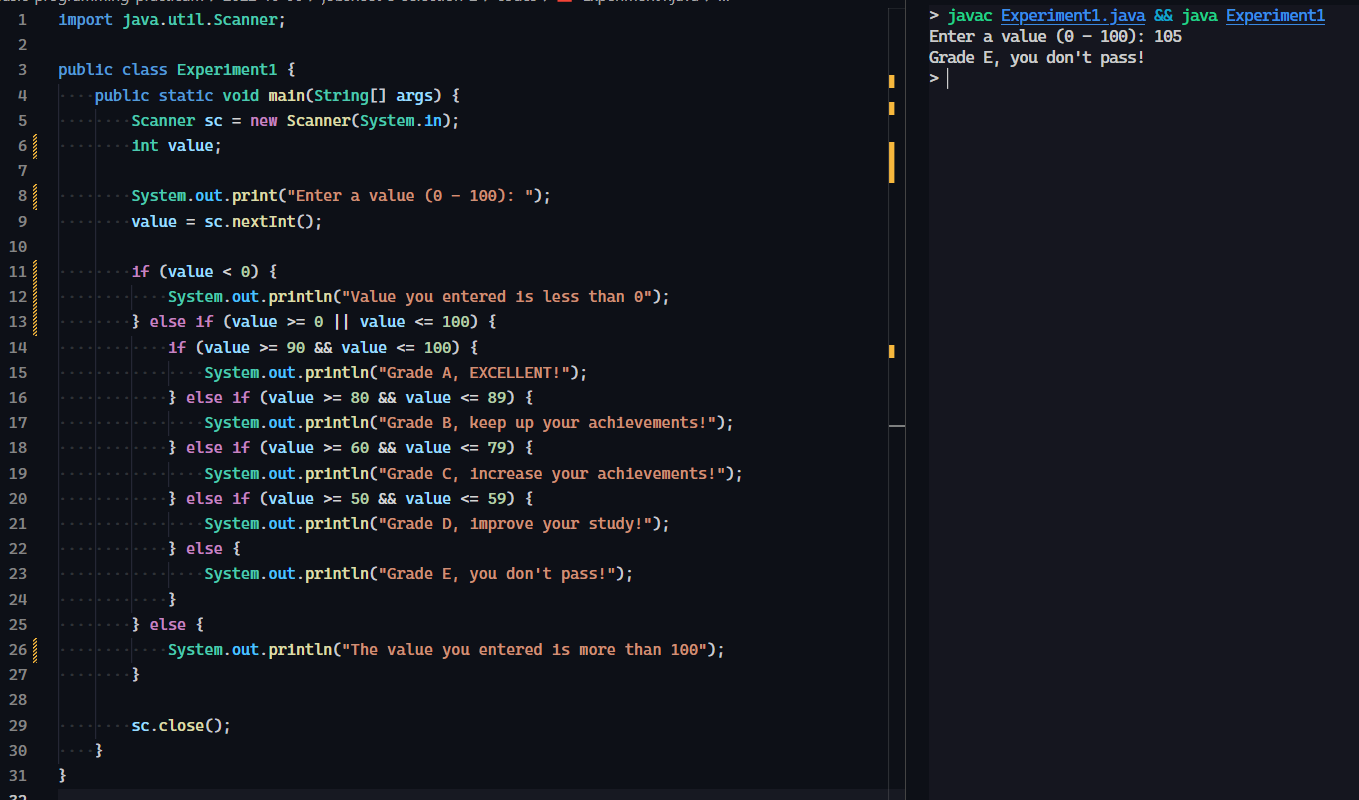
\includegraphics[width=\textwidth]{images/experiment1-or.png}
            \caption{Experiment 1 Modified Code and Output}
        \end{figure}

        Because the \texttt{||} condition checks if one of the expression is true.
        Since we set the \texttt{value} to be 105, the \texttt{value >= 0 || value <= 100} will be true Because
        value is greater than 0. Even though it's greater than 100, one of the condition is already true.
        The final result is \texttt{"Grade E, you don't pass!"} because there is no branch that handles a value greater than 100
        so it falls back to the default condition, which is inside the \texttt{else} branch.
    }
\end{enumerate}
\pagebreak
\subsection{Experiment 2}
\begin{enumerate}
    \item {
        Observe the following flowchart!
        
        \begin{figure}[h]
            \centering
            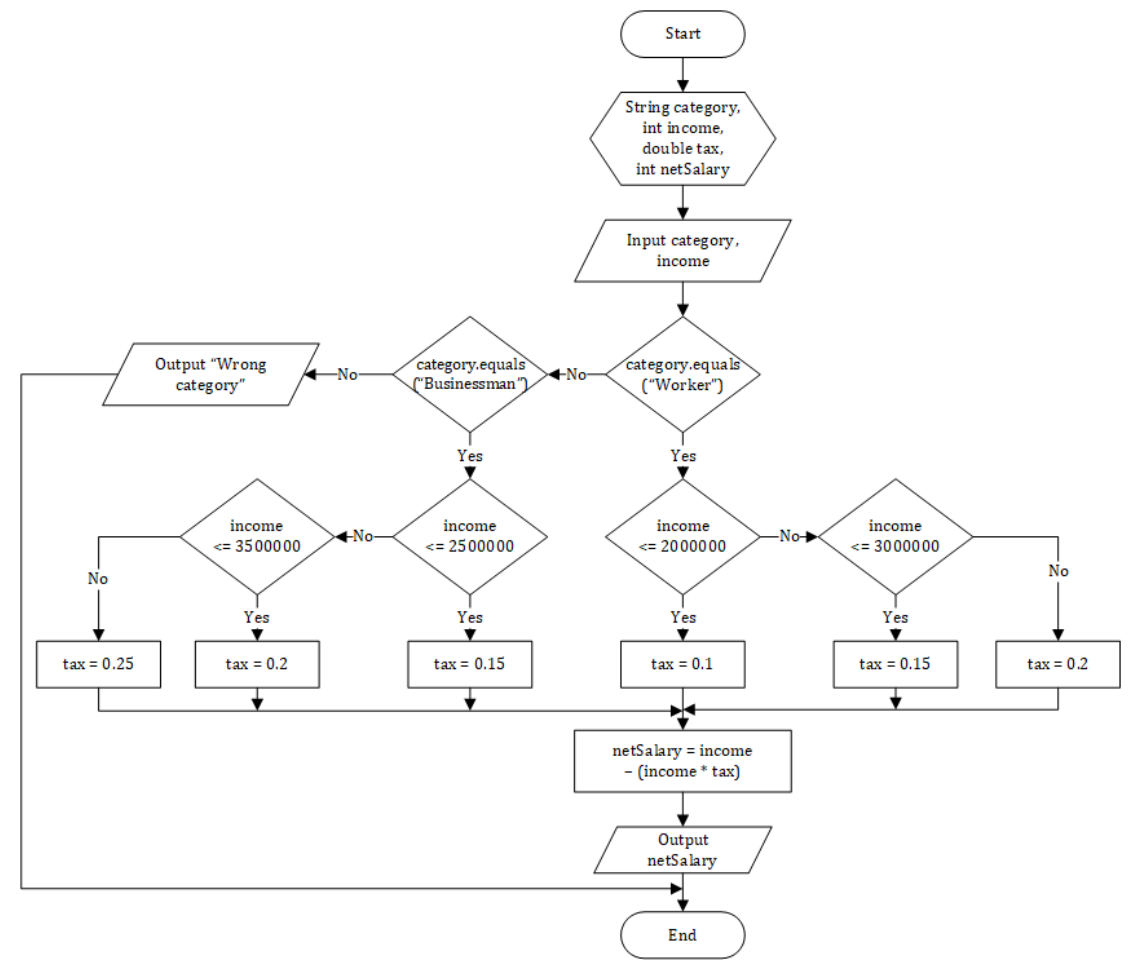
\includegraphics[width=\textwidth]{images/experiment2-flowchart.png}
            \caption{Experiment 2 Flowchart}
        \end{figure}

        The flowchart is used to calculate a person's net salary after taxes according to their
        category (worker and businessman) and the amount of income.
    }
    \item Open a text editor. Create a new file, name it \textbf{Nested2.java}
    \item Write the basic structure of the Java programming language which contains the \texttt{main()} function
    \item Add the \texttt{Scanner} library.
    \item Make a \texttt{Scanner} declaration with the name \texttt{sc}
    \pagebreak
    \item {
        Declare \texttt{category}, \texttt{income}, \texttt{netSalary}, and \texttt{tax} variables

        \begin{minted}[autogobble,fontsize=\small]{java}
            String category;
            int income, netSalary;
            double tax = 0;
        \end{minted}
    }
    \item {
        Write down the syntax for entering the value from keyboard

        \begin{minted}[autogobble,fontsize=\small]{java}
            System.out.print("Enter a category: ");
            category = sc.nextLine();
            System.out.print("Enter the amount of income: ");
            income = sc.nextInt();
        \end{minted}
    }
    \item {
        Create a nested selection structure. The first check is used to check the category (worker
        or businessman). Then a second check is carried out to determine the amount of tax
        based on the income that has been entered. Then add the program code to calculate the
        net salary received after taxes

        \begin{minted}[autogobble,fontsize=\small]{java}
            if (category.equalsIgnoreCase("worker")) {
                if (income <= 2000000) {
                    tax = 0.1;
                } else if (income <= 3000000) {
                    tax = 0.15;
                } else {
                    tax = 0.2;
                }
                netSalary = (int) (income - (income * tax));
                System.out.println("The net salary you will receive: " + netSalary);
            } else if (category.equalsIgnoreCase("businessman")) {
                if (income <= 2500000) {
                    tax = 0.15;
                } else if (income <= 3500000) {
                    tax = 0.2;
                } else {
                    tax = 0.25;
                }
                netSalary = (int) (income - (income * tax));
                System.out.println("The net salary you will receieve: " + netSalary);
            } else {
                System.out.println("The category you entered is wrong");
            }
        \end{minted}
    }
    \pagebreak
    \item {
        Compile and run the program. Observe the results!

        \begin{figure}[h]
            \centering
            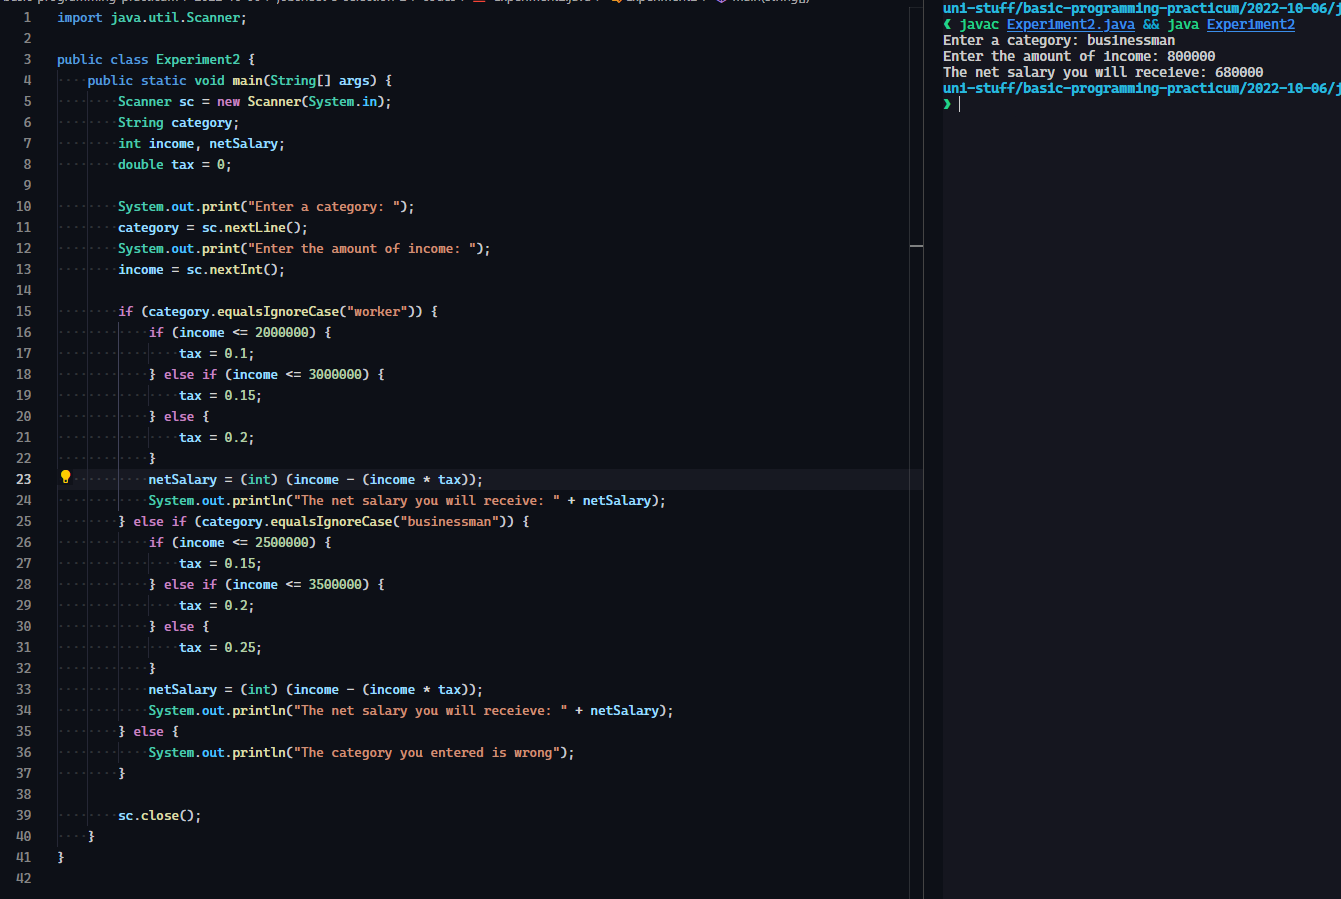
\includegraphics[width=\textwidth]{images/experiment2.png}
            \caption{Experiment 2 Code and Output}
        \end{figure}
    }
\end{enumerate}
\subsection*{Questions}
\begin{enumerate}
    \item {
        Run the program by entering category = worker and income = 2048485 using keyboard.
        Watch what happened! Why is the decimal number not displayed?

        \begin{figure}[h]
            \centering
            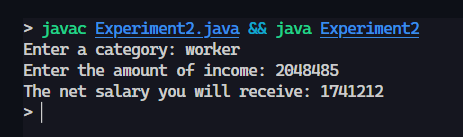
\includegraphics[width=.5\textwidth]{images/experiment2-output.png}
            \caption{Experiment 2 Output}
        \end{figure}

        The decimal number doesn't get displayed because we cast the final result back to integer.
        Specifically this part: 
        
        \begin{minted}[autogobble,fontsize=\small]{java}
            netSalary = (int) (income - (income * tax));
        \end{minted}
    }
    \pagebreak
    \item {
        Describe the function of \texttt{(int)} in the following syntax!

        \begin{minted}[autogobble,fontsize=\small]{java}
            netSalary = (int) (income - (income * tax));
        \end{minted}

        It is used to calculate the net salary by subtracting the income with the tax and then
        casting the result to an integer using \texttt{(int)}.
    }
    \item {
        Run the program by entering category = BUSINESSMAN and income = 2000000.
        Watch what happens! What are the uses of \texttt{equalsIgnoreCase}?

        \begin{figure}[h]
            \centering
            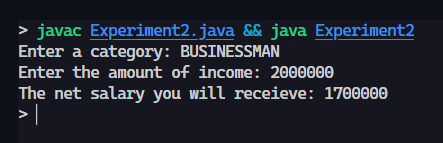
\includegraphics[width=.5\textwidth]{images/experiment2-uppercased.png}
            \caption{Experiment 2 Output}
        \end{figure}

        The \texttt{equalsIgnoreCase} is used to compare two string ignoring the case sensitivity.
        Which explains why \texttt{BUSINESSMAN} is still equals to \texttt{businessman}
    }
    \item {
        Change \texttt{equalsIgnoreCase} to \texttt{equals}, then run the program by entering 
        \texttt{category = BUSINESSMAN} and \texttt{income = 2000000}. Watch what happens!
        Why is the result like that? What are the uses of \texttt{equals}?

        The method \texttt{equals} compare two strings but it is case sensitive, while \texttt{equalsIgnoreCase} will
        ignore the case sensitivity. If we use \texttt{equals} to compare "businessman" with "BUSINESSMAN",
        it will be \texttt{false} but it will be \texttt{true} if we use \texttt{equalsIgnoreCase}.
    }
\end{enumerate}
\pagebreak
\section{Assignment}
\begin{enumerate}
    \item {
        Using three values that represent the lengths of the three sides of a triangle, determine
        whether the triangle is \textbf{equilateral} (all three sides are equal), \textbf{isosceles} (both sides are
        equal), or \textbf{arbitrary} (no sides are equal)!

        \begin{figure}[h]
            \centering
            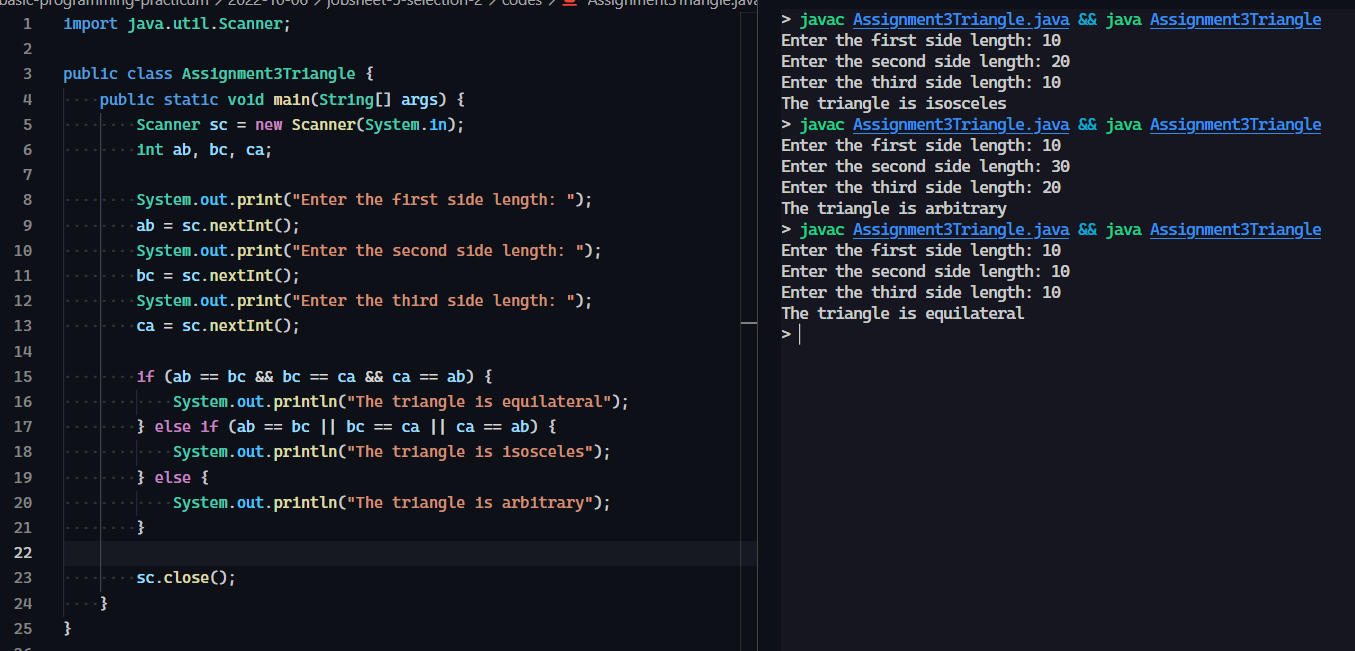
\includegraphics[width=\textwidth]{images/assignment3-triangle.png}
            \caption{Code and output to find triangle sides}
        \end{figure}
    }
    \pagebreak
    \item {
        A restaurant asks you to create a program for taking orders from the internet. The
        program you created asks the user to enter a food name and price. After that, the user is
        offered to use express delivery. If the user refuses, the delivery type used is regular
        delivery. Regular delivery costs for food less than IDR 100,000 are IDR 20,000, while for
        food prices equal to or more than IDR 100,000 the delivery cost is IDR 30,000. For express
        delivery, add an additional fee of IDR 25,000 from the standard regular shipping cost.
        Show a receipt containing the name of the food purchased + price, shipping costs and the
        total to be paid!

        \begin{figure}[h]
            \centering
            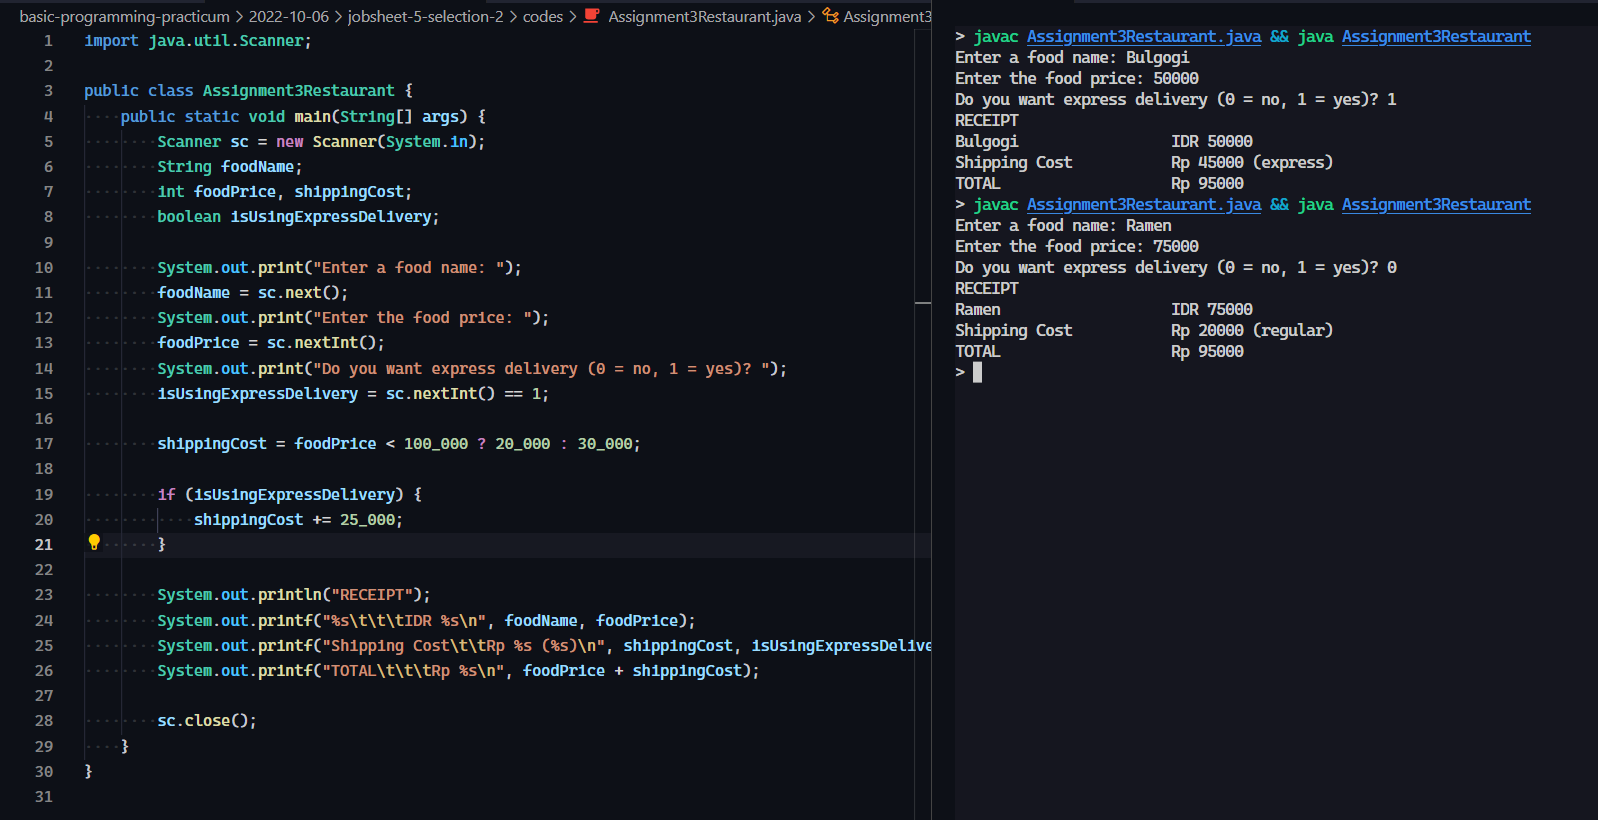
\includegraphics[width=\textwidth]{images/assignment3-restaurant.png}
            \caption{Code and output to calculate total price for a restaurant}
        \end{figure}
    }
\end{enumerate}

\end{document}

